% Created by tikzDevice version 0.6.2-92-0ad2792 on 2013-04-07 23:44:31
% !TEX encoding = UTF-8 Unicode
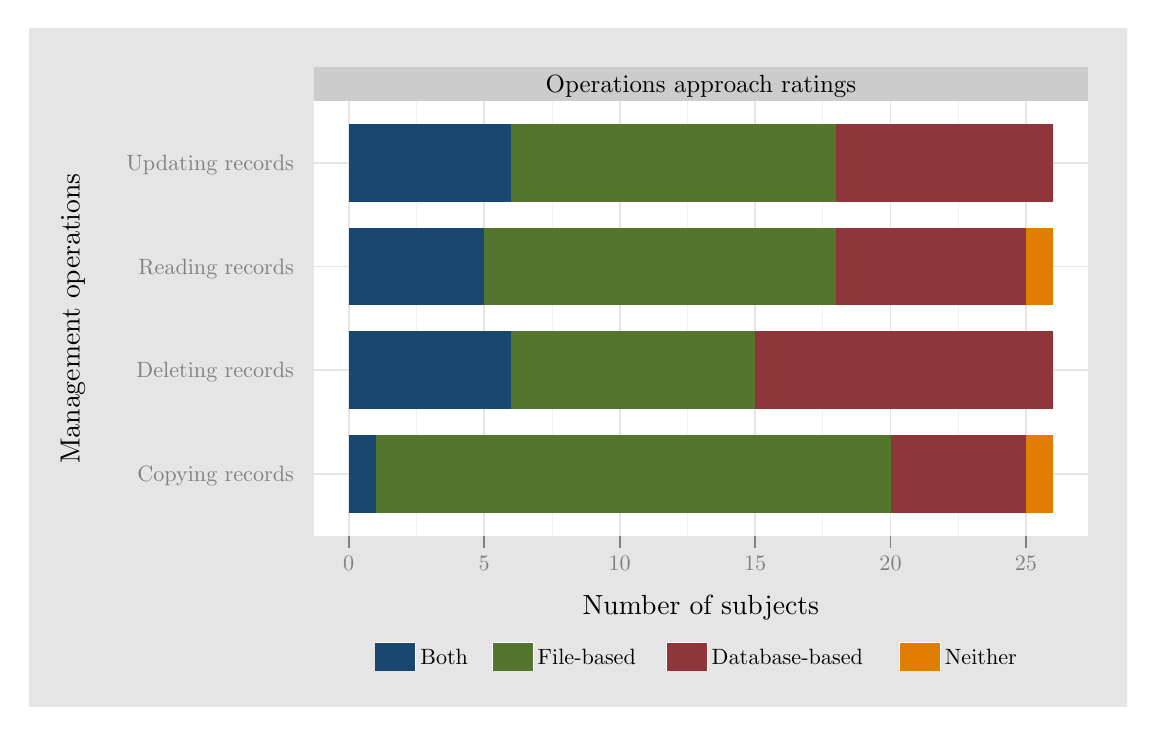
\begin{tikzpicture}[x=1pt,y=1pt]
\definecolor[named]{fillColor}{rgb}{1.00,1.00,1.00}
\path[use as bounding box,fill=fillColor,fill opacity=0.00] (0,0) rectangle (397.48,245.72);
\begin{scope}
\path[clip] (  0.00,  0.00) rectangle (397.48,245.72);
\definecolor[named]{drawColor}{rgb}{1.00,1.00,1.00}
\definecolor[named]{fillColor}{rgb}{0.90,0.90,0.90}

\path[draw=drawColor,line width= 0.6pt,line join=round,line cap=round,fill=fillColor] (  0.00,  0.00) rectangle (397.48,245.72);
\end{scope}
\begin{scope}
\path[clip] (103.30, 62.05) rectangle (383.26,219.27);
\definecolor[named]{fillColor}{rgb}{1.00,1.00,1.00}

\path[fill=fillColor] (103.30, 62.05) rectangle (383.26,219.27);
\definecolor[named]{drawColor}{rgb}{0.95,0.95,0.95}

\path[draw=drawColor,line width= 0.3pt,line join=round] (140.50, 62.05) --
	(140.50,219.27);

\path[draw=drawColor,line width= 0.3pt,line join=round] (189.44, 62.05) --
	(189.44,219.27);

\path[draw=drawColor,line width= 0.3pt,line join=round] (238.39, 62.05) --
	(238.39,219.27);

\path[draw=drawColor,line width= 0.3pt,line join=round] (287.33, 62.05) --
	(287.33,219.27);

\path[draw=drawColor,line width= 0.3pt,line join=round] (336.27, 62.05) --
	(336.27,219.27);
\definecolor[named]{drawColor}{rgb}{0.90,0.90,0.90}

\path[draw=drawColor,line width= 0.6pt,line join=round] (103.30, 84.51) --
	(383.26, 84.51);

\path[draw=drawColor,line width= 0.6pt,line join=round] (103.30,121.94) --
	(383.26,121.94);

\path[draw=drawColor,line width= 0.6pt,line join=round] (103.30,159.38) --
	(383.26,159.38);

\path[draw=drawColor,line width= 0.6pt,line join=round] (103.30,196.81) --
	(383.26,196.81);

\path[draw=drawColor,line width= 0.6pt,line join=round] (116.03, 62.05) --
	(116.03,219.27);

\path[draw=drawColor,line width= 0.6pt,line join=round] (164.97, 62.05) --
	(164.97,219.27);

\path[draw=drawColor,line width= 0.6pt,line join=round] (213.92, 62.05) --
	(213.92,219.27);

\path[draw=drawColor,line width= 0.6pt,line join=round] (262.86, 62.05) --
	(262.86,219.27);

\path[draw=drawColor,line width= 0.6pt,line join=round] (311.80, 62.05) --
	(311.80,219.27);

\path[draw=drawColor,line width= 0.6pt,line join=round] (360.74, 62.05) --
	(360.74,219.27);
\definecolor[named]{fillColor}{rgb}{0.10,0.28,0.44}

\path[fill=fillColor] (116.03, 70.47) rectangle (125.82, 98.55);
\definecolor[named]{fillColor}{rgb}{0.33,0.46,0.18}

\path[fill=fillColor] (125.82, 70.47) rectangle (311.80, 98.55);
\definecolor[named]{fillColor}{rgb}{0.56,0.21,0.23}

\path[fill=fillColor] (311.80, 70.47) rectangle (360.74, 98.55);
\definecolor[named]{fillColor}{rgb}{0.89,0.49,0.00}

\path[fill=fillColor] (360.74, 70.47) rectangle (370.53, 98.55);
\definecolor[named]{fillColor}{rgb}{0.10,0.28,0.44}

\path[fill=fillColor] (116.03,107.90) rectangle (174.76,135.98);
\definecolor[named]{fillColor}{rgb}{0.33,0.46,0.18}

\path[fill=fillColor] (174.76,107.90) rectangle (262.86,135.98);
\definecolor[named]{fillColor}{rgb}{0.56,0.21,0.23}

\path[fill=fillColor] (262.86,107.90) rectangle (370.53,135.98);
\definecolor[named]{fillColor}{rgb}{0.89,0.49,0.00}

\path[fill=fillColor] (370.53,107.90) rectangle (370.53,135.98);
\definecolor[named]{fillColor}{rgb}{0.10,0.28,0.44}

\path[fill=fillColor] (116.03,145.34) rectangle (164.97,173.41);
\definecolor[named]{fillColor}{rgb}{0.33,0.46,0.18}

\path[fill=fillColor] (164.97,145.34) rectangle (292.22,173.41);
\definecolor[named]{fillColor}{rgb}{0.56,0.21,0.23}

\path[fill=fillColor] (292.22,145.34) rectangle (360.74,173.41);
\definecolor[named]{fillColor}{rgb}{0.89,0.49,0.00}

\path[fill=fillColor] (360.74,145.34) rectangle (370.53,173.41);
\definecolor[named]{fillColor}{rgb}{0.10,0.28,0.44}

\path[fill=fillColor] (116.03,182.77) rectangle (174.76,210.85);
\definecolor[named]{fillColor}{rgb}{0.33,0.46,0.18}

\path[fill=fillColor] (174.76,182.77) rectangle (292.22,210.85);
\definecolor[named]{fillColor}{rgb}{0.56,0.21,0.23}

\path[fill=fillColor] (292.22,182.77) rectangle (370.53,210.85);
\definecolor[named]{fillColor}{rgb}{0.89,0.49,0.00}

\path[fill=fillColor] (370.53,182.77) rectangle (370.53,210.85);
\end{scope}
\begin{scope}
\path[clip] (  0.00,  0.00) rectangle (397.48,245.72);
\definecolor[named]{fillColor}{rgb}{0.80,0.80,0.80}

\path[fill=fillColor] (103.30,219.27) rectangle (383.26,231.49);
\definecolor[named]{drawColor}{rgb}{0.00,0.00,0.00}

\node[text=drawColor,anchor=base,inner sep=0pt, outer sep=0pt, scale=  0.90] at (243.28,222.28) {Operations approach ratings};
\end{scope}
\begin{scope}
\path[clip] (  0.00,  0.00) rectangle (397.48,245.72);
\definecolor[named]{drawColor}{rgb}{0.50,0.50,0.50}

\node[text=drawColor,anchor=base east,inner sep=0pt, outer sep=0pt, scale=  0.80] at ( 96.19, 81.75) {Copying records};

\node[text=drawColor,anchor=base east,inner sep=0pt, outer sep=0pt, scale=  0.80] at ( 96.19,119.19) {Deleting records};

\node[text=drawColor,anchor=base east,inner sep=0pt, outer sep=0pt, scale=  0.80] at ( 96.19,156.62) {Reading records};

\node[text=drawColor,anchor=base east,inner sep=0pt, outer sep=0pt, scale=  0.80] at ( 96.19,194.06) {Updating records};
\end{scope}
\begin{scope}
\path[clip] (  0.00,  0.00) rectangle (397.48,245.72);
\definecolor[named]{drawColor}{rgb}{0.50,0.50,0.50}

\path[draw=drawColor,line width= 0.6pt,line join=round] (116.03, 57.78) --
	(116.03, 62.05);

\path[draw=drawColor,line width= 0.6pt,line join=round] (164.97, 57.78) --
	(164.97, 62.05);

\path[draw=drawColor,line width= 0.6pt,line join=round] (213.92, 57.78) --
	(213.92, 62.05);

\path[draw=drawColor,line width= 0.6pt,line join=round] (262.86, 57.78) --
	(262.86, 62.05);

\path[draw=drawColor,line width= 0.6pt,line join=round] (311.80, 57.78) --
	(311.80, 62.05);

\path[draw=drawColor,line width= 0.6pt,line join=round] (360.74, 57.78) --
	(360.74, 62.05);
\end{scope}
\begin{scope}
\path[clip] (  0.00,  0.00) rectangle (397.48,245.72);
\definecolor[named]{drawColor}{rgb}{0.50,0.50,0.50}

\node[text=drawColor,anchor=base,inner sep=0pt, outer sep=0pt, scale=  0.80] at (116.03, 49.42) {0};

\node[text=drawColor,anchor=base,inner sep=0pt, outer sep=0pt, scale=  0.80] at (164.97, 49.42) {5};

\node[text=drawColor,anchor=base,inner sep=0pt, outer sep=0pt, scale=  0.80] at (213.92, 49.42) {10};

\node[text=drawColor,anchor=base,inner sep=0pt, outer sep=0pt, scale=  0.80] at (262.86, 49.42) {15};

\node[text=drawColor,anchor=base,inner sep=0pt, outer sep=0pt, scale=  0.80] at (311.80, 49.42) {20};

\node[text=drawColor,anchor=base,inner sep=0pt, outer sep=0pt, scale=  0.80] at (360.74, 49.42) {25};
\end{scope}
\begin{scope}
\path[clip] (  0.00,  0.00) rectangle (397.48,245.72);
\definecolor[named]{drawColor}{rgb}{0.00,0.00,0.00}

\node[text=drawColor,anchor=base,inner sep=0pt, outer sep=0pt, scale=  1.00] at (243.28, 33.50) {Number of subjects};
\end{scope}
\begin{scope}
\path[clip] (  0.00,  0.00) rectangle (397.48,245.72);
\definecolor[named]{drawColor}{rgb}{0.00,0.00,0.00}

\node[text=drawColor,rotate= 90.00,anchor=base,inner sep=0pt, outer sep=0pt, scale=  1.00] at ( 18.80,140.66) {Management operations};
\end{scope}
\begin{scope}
\path[clip] (  0.00,  0.00) rectangle (397.48,245.72);
\definecolor[named]{fillColor}{rgb}{0.90,0.90,0.90}

\path[fill=fillColor] (117.75,  9.15) rectangle (368.81, 27.65);
\end{scope}
\begin{scope}
\path[clip] (  0.00,  0.00) rectangle (397.48,245.72);
\definecolor[named]{drawColor}{rgb}{1.00,1.00,1.00}
\definecolor[named]{fillColor}{rgb}{1.00,1.00,1.00}

\path[draw=drawColor,line width= 0.6pt,line join=round,line cap=round,fill=fillColor] (125.63, 13.42) rectangle (140.08, 23.38);
\end{scope}
\begin{scope}
\path[clip] (  0.00,  0.00) rectangle (397.48,245.72);
\definecolor[named]{fillColor}{rgb}{0.10,0.28,0.44}

\path[fill=fillColor] (125.63, 13.42) rectangle (140.08, 23.38);

\path[] (125.63, 13.42) --
	(140.08, 23.38);
\end{scope}
\begin{scope}
\path[clip] (  0.00,  0.00) rectangle (397.48,245.72);
\definecolor[named]{drawColor}{rgb}{1.00,1.00,1.00}
\definecolor[named]{fillColor}{rgb}{1.00,1.00,1.00}

\path[draw=drawColor,line width= 0.6pt,line join=round,line cap=round,fill=fillColor] (168.03, 13.42) rectangle (182.48, 23.38);
\end{scope}
\begin{scope}
\path[clip] (  0.00,  0.00) rectangle (397.48,245.72);
\definecolor[named]{fillColor}{rgb}{0.33,0.46,0.18}

\path[fill=fillColor] (168.03, 13.42) rectangle (182.48, 23.38);

\path[] (168.03, 13.42) --
	(182.48, 23.38);
\end{scope}
\begin{scope}
\path[clip] (  0.00,  0.00) rectangle (397.48,245.72);
\definecolor[named]{drawColor}{rgb}{1.00,1.00,1.00}
\definecolor[named]{fillColor}{rgb}{1.00,1.00,1.00}

\path[draw=drawColor,line width= 0.6pt,line join=round,line cap=round,fill=fillColor] (230.91, 13.42) rectangle (245.36, 23.38);
\end{scope}
\begin{scope}
\path[clip] (  0.00,  0.00) rectangle (397.48,245.72);
\definecolor[named]{fillColor}{rgb}{0.56,0.21,0.23}

\path[fill=fillColor] (230.91, 13.42) rectangle (245.36, 23.38);

\path[] (230.91, 13.42) --
	(245.36, 23.38);
\end{scope}
\begin{scope}
\path[clip] (  0.00,  0.00) rectangle (397.48,245.72);
\definecolor[named]{drawColor}{rgb}{1.00,1.00,1.00}
\definecolor[named]{fillColor}{rgb}{1.00,1.00,1.00}

\path[draw=drawColor,line width= 0.6pt,line join=round,line cap=round,fill=fillColor] (315.16, 13.42) rectangle (329.61, 23.38);
\end{scope}
\begin{scope}
\path[clip] (  0.00,  0.00) rectangle (397.48,245.72);
\definecolor[named]{fillColor}{rgb}{0.89,0.49,0.00}

\path[fill=fillColor] (315.16, 13.42) rectangle (329.61, 23.38);

\path[] (315.16, 13.42) --
	(329.61, 23.38);
\end{scope}
\begin{scope}
\path[clip] (  0.00,  0.00) rectangle (397.48,245.72);
\definecolor[named]{drawColor}{rgb}{0.00,0.00,0.00}

\node[text=drawColor,anchor=base west,inner sep=0pt, outer sep=0pt, scale=  0.80] at (141.89, 15.64) {Both $\;\;$};
\end{scope}
\begin{scope}
\path[clip] (  0.00,  0.00) rectangle (397.48,245.72);
\definecolor[named]{drawColor}{rgb}{0.00,0.00,0.00}

\node[text=drawColor,anchor=base west,inner sep=0pt, outer sep=0pt, scale=  0.80] at (184.29, 15.64) {File-based $\;\;\;$};
\end{scope}
\begin{scope}
\path[clip] (  0.00,  0.00) rectangle (397.48,245.72);
\definecolor[named]{drawColor}{rgb}{0.00,0.00,0.00}

\node[text=drawColor,anchor=base west,inner sep=0pt, outer sep=0pt, scale=  0.80] at (247.17, 15.64) {Database-based $\;\;\;\;$};
\end{scope}
\begin{scope}
\path[clip] (  0.00,  0.00) rectangle (397.48,245.72);
\definecolor[named]{drawColor}{rgb}{0.00,0.00,0.00}

\node[text=drawColor,anchor=base west,inner sep=0pt, outer sep=0pt, scale=  0.80] at (331.42, 15.64) {Neither $\;\;$};
\end{scope}
\end{tikzpicture}
